% !TEX encoding = UTF-8 Unicode
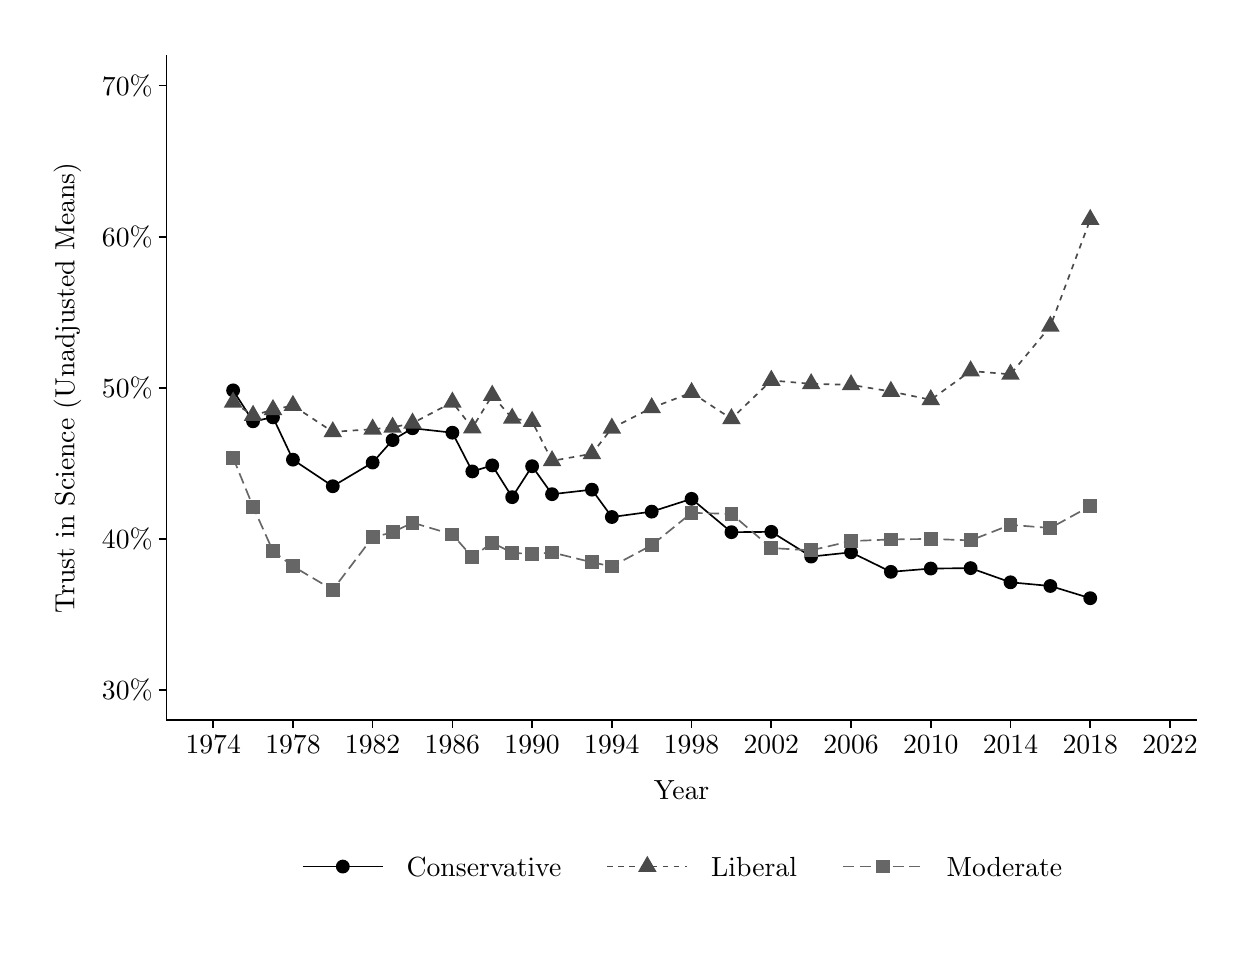
\begin{tikzpicture}[x=1pt,y=1pt]
\definecolor{fillColor}{RGB}{255,255,255}
\path[use as bounding box,fill=fillColor,fill opacity=0.00] (0,0) rectangle (432.48,324.36);
\begin{scope}
\path[clip] (  0.00,  0.00) rectangle (432.48,324.36);
\definecolor{fillColor}{RGB}{255,255,255}

\path[fill=fillColor] ( -0.00,  0.00) rectangle (432.48,324.36);
\end{scope}
\begin{scope}
\path[clip] ( 50.11, 74.07) rectangle (422.48,314.36);
\definecolor{fillColor}{RGB}{255,255,255}

\path[fill=fillColor] ( 50.11, 74.07) rectangle (422.48,314.36);
\definecolor{drawColor}{RGB}{0,0,0}

\path[draw=drawColor,line width= 0.6pt,line join=round] ( 74.24,193.29) --
	( 81.44,182.12) --
	( 88.64,183.54) --
	( 95.85,168.26) --
	(110.25,158.65) --
	(124.66,167.22) --
	(131.86,175.33) --
	(139.06,179.60) --
	(153.47,178.00) --
	(160.67,164.00) --
	(167.87,166.18) --
	(175.07,154.71) --
	(182.28,165.89) --
	(189.48,155.78) --
	(203.88,157.42) --
	(211.09,147.53) --
	(225.49,149.48) --
	(239.90,154.10) --
	(254.30,142.05) --
	(268.71,142.18) --
	(283.11,133.24) --
	(297.52,134.77) --
	(311.92,127.72) --
	(326.33,128.91) --
	(340.73,129.06) --
	(355.14,123.94) --
	(369.54,122.61) --
	(383.95,118.20);
\definecolor{drawColor}{gray}{0.29}

\path[draw=drawColor,line width= 0.6pt,dash pattern=on 2pt off 2pt ,line join=round] ( 74.24,189.03) --
	( 81.44,184.23) --
	( 88.64,186.31) --
	( 95.85,187.82) --
	(110.25,178.30) --
	(124.66,179.28) --
	(131.86,179.93) --
	(139.06,181.43) --
	(153.47,189.01) --
	(160.67,179.73) --
	(167.87,191.49) --
	(175.07,183.18) --
	(182.28,182.06) --
	(189.48,167.83) --
	(203.88,170.39) --
	(211.09,179.61) --
	(225.49,186.99) --
	(239.90,192.48) --
	(254.30,183.03) --
	(268.71,196.89) --
	(283.11,195.66) --
	(297.52,195.29) --
	(311.92,192.90) --
	(326.33,189.90) --
	(340.73,200.30) --
	(355.14,199.09) --
	(369.54,216.46) --
	(383.95,255.00);
\definecolor{drawColor}{gray}{0.40}

\path[draw=drawColor,line width= 0.6pt,dash pattern=on 4pt off 2pt ,line join=round] ( 74.24,168.91) --
	( 81.44,151.28) --
	( 88.64,135.23) --
	( 95.85,129.72) --
	(110.25,121.24) --
	(124.66,140.21) --
	(131.86,141.99) --
	(139.06,145.49) --
	(153.47,141.23) --
	(160.67,133.07) --
	(167.87,138.26) --
	(175.07,134.61) --
	(182.28,134.12) --
	(189.48,134.73) --
	(203.88,131.18) --
	(211.09,129.68) --
	(225.49,137.35) --
	(239.90,149.03) --
	(254.30,148.68) --
	(268.71,136.31) --
	(283.11,135.50) --
	(297.52,138.84) --
	(311.92,139.43) --
	(326.33,139.62) --
	(340.73,139.09) --
	(355.14,144.71) --
	(369.54,143.56) --
	(383.95,151.46);
\definecolor{fillColor}{RGB}{0,0,0}

\path[fill=fillColor] ( 74.24,193.29) circle (  2.50);
\definecolor{fillColor}{gray}{0.29}

\path[fill=fillColor] ( 74.24,192.91) --
	( 77.60,187.09) --
	( 70.87,187.09) --
	cycle;
\definecolor{fillColor}{gray}{0.40}

\path[fill=fillColor] ( 71.74,166.41) --
	( 76.74,166.41) --
	( 76.74,171.41) --
	( 71.74,171.41) --
	cycle;
\definecolor{fillColor}{RGB}{0,0,0}

\path[fill=fillColor] ( 81.44,182.12) circle (  2.50);
\definecolor{fillColor}{gray}{0.29}

\path[fill=fillColor] ( 81.44,188.11) --
	( 84.80,182.28) --
	( 78.08,182.28) --
	cycle;
\definecolor{fillColor}{gray}{0.40}

\path[fill=fillColor] ( 78.94,148.78) --
	( 83.94,148.78) --
	( 83.94,153.77) --
	( 78.94,153.77) --
	cycle;
\definecolor{fillColor}{RGB}{0,0,0}

\path[fill=fillColor] ( 88.64,183.54) circle (  2.50);
\definecolor{fillColor}{gray}{0.29}

\path[fill=fillColor] ( 88.64,190.19) --
	( 92.01,184.37) --
	( 85.28,184.37) --
	cycle;
\definecolor{fillColor}{gray}{0.40}

\path[fill=fillColor] ( 86.15,132.73) --
	( 91.14,132.73) --
	( 91.14,137.73) --
	( 86.15,137.73) --
	cycle;
\definecolor{fillColor}{RGB}{0,0,0}

\path[fill=fillColor] ( 95.85,168.26) circle (  2.50);
\definecolor{fillColor}{gray}{0.29}

\path[fill=fillColor] ( 95.85,191.70) --
	( 99.21,185.88) --
	( 92.48,185.88) --
	cycle;
\definecolor{fillColor}{gray}{0.40}

\path[fill=fillColor] ( 93.35,127.22) --
	( 98.34,127.22) --
	( 98.34,132.21) --
	( 93.35,132.21) --
	cycle;
\definecolor{fillColor}{RGB}{0,0,0}

\path[fill=fillColor] (110.25,158.65) circle (  2.50);
\definecolor{fillColor}{gray}{0.29}

\path[fill=fillColor] (110.25,182.19) --
	(113.62,176.36) --
	(106.89,176.36) --
	cycle;
\definecolor{fillColor}{gray}{0.40}

\path[fill=fillColor] (107.75,118.74) --
	(112.75,118.74) --
	(112.75,123.74) --
	(107.75,123.74) --
	cycle;
\definecolor{fillColor}{RGB}{0,0,0}

\path[fill=fillColor] (124.66,167.22) circle (  2.50);
\definecolor{fillColor}{gray}{0.29}

\path[fill=fillColor] (124.66,183.16) --
	(128.02,177.34) --
	(121.29,177.34) --
	cycle;
\definecolor{fillColor}{gray}{0.40}

\path[fill=fillColor] (122.16,137.71) --
	(127.15,137.71) --
	(127.15,142.70) --
	(122.16,142.70) --
	cycle;
\definecolor{fillColor}{RGB}{0,0,0}

\path[fill=fillColor] (131.86,175.33) circle (  2.50);
\definecolor{fillColor}{gray}{0.29}

\path[fill=fillColor] (131.86,183.81) --
	(135.22,177.99) --
	(128.50,177.99) --
	cycle;
\definecolor{fillColor}{gray}{0.40}

\path[fill=fillColor] (129.36,139.49) --
	(134.36,139.49) --
	(134.36,144.49) --
	(129.36,144.49) --
	cycle;
\definecolor{fillColor}{RGB}{0,0,0}

\path[fill=fillColor] (139.06,179.60) circle (  2.50);
\definecolor{fillColor}{gray}{0.29}

\path[fill=fillColor] (139.06,185.31) --
	(142.43,179.49) --
	(135.70,179.49) --
	cycle;
\definecolor{fillColor}{gray}{0.40}

\path[fill=fillColor] (136.56,142.99) --
	(141.56,142.99) --
	(141.56,147.99) --
	(136.56,147.99) --
	cycle;
\definecolor{fillColor}{RGB}{0,0,0}

\path[fill=fillColor] (153.47,178.00) circle (  2.50);
\definecolor{fillColor}{gray}{0.29}

\path[fill=fillColor] (153.47,192.89) --
	(156.83,187.07) --
	(150.10,187.07) --
	cycle;
\definecolor{fillColor}{gray}{0.40}

\path[fill=fillColor] (150.97,138.73) --
	(155.96,138.73) --
	(155.96,143.72) --
	(150.97,143.72) --
	cycle;
\definecolor{fillColor}{RGB}{0,0,0}

\path[fill=fillColor] (160.67,164.00) circle (  2.50);
\definecolor{fillColor}{gray}{0.29}

\path[fill=fillColor] (160.67,183.61) --
	(164.03,177.79) --
	(157.31,177.79) --
	cycle;
\definecolor{fillColor}{gray}{0.40}

\path[fill=fillColor] (158.17,130.57) --
	(163.17,130.57) --
	(163.17,135.57) --
	(158.17,135.57) --
	cycle;
\definecolor{fillColor}{RGB}{0,0,0}

\path[fill=fillColor] (167.87,166.18) circle (  2.50);
\definecolor{fillColor}{gray}{0.29}

\path[fill=fillColor] (167.87,195.37) --
	(171.24,189.54) --
	(164.51,189.54) --
	cycle;
\definecolor{fillColor}{gray}{0.40}

\path[fill=fillColor] (165.37,135.77) --
	(170.37,135.77) --
	(170.37,140.76) --
	(165.37,140.76) --
	cycle;
\definecolor{fillColor}{RGB}{0,0,0}

\path[fill=fillColor] (175.07,154.71) circle (  2.50);
\definecolor{fillColor}{gray}{0.29}

\path[fill=fillColor] (175.07,187.07) --
	(178.44,181.24) --
	(171.71,181.24) --
	cycle;
\definecolor{fillColor}{gray}{0.40}

\path[fill=fillColor] (172.58,132.11) --
	(177.57,132.11) --
	(177.57,137.11) --
	(172.58,137.11) --
	cycle;
\definecolor{fillColor}{RGB}{0,0,0}

\path[fill=fillColor] (182.28,165.89) circle (  2.50);
\definecolor{fillColor}{gray}{0.29}

\path[fill=fillColor] (182.28,185.95) --
	(185.64,180.12) --
	(178.91,180.12) --
	cycle;
\definecolor{fillColor}{gray}{0.40}

\path[fill=fillColor] (179.78,131.62) --
	(184.77,131.62) --
	(184.77,136.61) --
	(179.78,136.61) --
	cycle;
\definecolor{fillColor}{RGB}{0,0,0}

\path[fill=fillColor] (189.48,155.78) circle (  2.50);
\definecolor{fillColor}{gray}{0.29}

\path[fill=fillColor] (189.48,171.71) --
	(192.84,165.89) --
	(186.12,165.89) --
	cycle;
\definecolor{fillColor}{gray}{0.40}

\path[fill=fillColor] (186.98,132.23) --
	(191.98,132.23) --
	(191.98,137.22) --
	(186.98,137.22) --
	cycle;
\definecolor{fillColor}{RGB}{0,0,0}

\path[fill=fillColor] (203.88,157.42) circle (  2.50);
\definecolor{fillColor}{gray}{0.29}

\path[fill=fillColor] (203.88,174.27) --
	(207.25,168.45) --
	(200.52,168.45) --
	cycle;
\definecolor{fillColor}{gray}{0.40}

\path[fill=fillColor] (201.39,128.68) --
	(206.38,128.68) --
	(206.38,133.68) --
	(201.39,133.68) --
	cycle;
\definecolor{fillColor}{RGB}{0,0,0}

\path[fill=fillColor] (211.09,147.53) circle (  2.50);
\definecolor{fillColor}{gray}{0.29}

\path[fill=fillColor] (211.09,183.50) --
	(214.45,177.67) --
	(207.72,177.67) --
	cycle;
\definecolor{fillColor}{gray}{0.40}

\path[fill=fillColor] (208.59,127.18) --
	(213.58,127.18) --
	(213.58,132.18) --
	(208.59,132.18) --
	cycle;
\definecolor{fillColor}{RGB}{0,0,0}

\path[fill=fillColor] (225.49,149.48) circle (  2.50);
\definecolor{fillColor}{gray}{0.29}

\path[fill=fillColor] (225.49,190.87) --
	(228.86,185.04) --
	(222.13,185.04) --
	cycle;
\definecolor{fillColor}{gray}{0.40}

\path[fill=fillColor] (222.99,134.86) --
	(227.99,134.86) --
	(227.99,139.85) --
	(222.99,139.85) --
	cycle;
\definecolor{fillColor}{RGB}{0,0,0}

\path[fill=fillColor] (239.90,154.10) circle (  2.50);
\definecolor{fillColor}{gray}{0.29}

\path[fill=fillColor] (239.90,196.36) --
	(243.26,190.54) --
	(236.53,190.54) --
	cycle;
\definecolor{fillColor}{gray}{0.40}

\path[fill=fillColor] (237.40,146.53) --
	(242.39,146.53) --
	(242.39,151.53) --
	(237.40,151.53) --
	cycle;
\definecolor{fillColor}{RGB}{0,0,0}

\path[fill=fillColor] (254.30,142.05) circle (  2.50);
\definecolor{fillColor}{gray}{0.29}

\path[fill=fillColor] (254.30,186.92) --
	(257.67,181.09) --
	(250.94,181.09) --
	cycle;
\definecolor{fillColor}{gray}{0.40}

\path[fill=fillColor] (251.80,146.18) --
	(256.80,146.18) --
	(256.80,151.18) --
	(251.80,151.18) --
	cycle;
\definecolor{fillColor}{RGB}{0,0,0}

\path[fill=fillColor] (268.71,142.18) circle (  2.50);
\definecolor{fillColor}{gray}{0.29}

\path[fill=fillColor] (268.71,200.77) --
	(272.07,194.94) --
	(265.34,194.94) --
	cycle;
\definecolor{fillColor}{gray}{0.40}

\path[fill=fillColor] (266.21,133.81) --
	(271.21,133.81) --
	(271.21,138.81) --
	(266.21,138.81) --
	cycle;
\definecolor{fillColor}{RGB}{0,0,0}

\path[fill=fillColor] (283.11,133.24) circle (  2.50);
\definecolor{fillColor}{gray}{0.29}

\path[fill=fillColor] (283.11,199.55) --
	(286.48,193.72) --
	(279.75,193.72) --
	cycle;
\definecolor{fillColor}{gray}{0.40}

\path[fill=fillColor] (280.61,133.01) --
	(285.61,133.01) --
	(285.61,138.00) --
	(280.61,138.00) --
	cycle;
\definecolor{fillColor}{RGB}{0,0,0}

\path[fill=fillColor] (297.52,134.77) circle (  2.50);
\definecolor{fillColor}{gray}{0.29}

\path[fill=fillColor] (297.52,199.17) --
	(300.88,193.35) --
	(294.15,193.35) --
	cycle;
\definecolor{fillColor}{gray}{0.40}

\path[fill=fillColor] (295.02,136.34) --
	(300.02,136.34) --
	(300.02,141.34) --
	(295.02,141.34) --
	cycle;
\definecolor{fillColor}{RGB}{0,0,0}

\path[fill=fillColor] (311.92,127.72) circle (  2.50);
\definecolor{fillColor}{gray}{0.29}

\path[fill=fillColor] (311.92,196.78) --
	(315.29,190.95) --
	(308.56,190.95) --
	cycle;
\definecolor{fillColor}{gray}{0.40}

\path[fill=fillColor] (309.43,136.93) --
	(314.42,136.93) --
	(314.42,141.93) --
	(309.43,141.93) --
	cycle;
\definecolor{fillColor}{RGB}{0,0,0}

\path[fill=fillColor] (326.33,128.91) circle (  2.50);
\definecolor{fillColor}{gray}{0.29}

\path[fill=fillColor] (326.33,193.78) --
	(329.69,187.96) --
	(322.96,187.96) --
	cycle;
\definecolor{fillColor}{gray}{0.40}

\path[fill=fillColor] (323.83,137.12) --
	(328.83,137.12) --
	(328.83,142.11) --
	(323.83,142.11) --
	cycle;
\definecolor{fillColor}{RGB}{0,0,0}

\path[fill=fillColor] (340.73,129.06) circle (  2.50);
\definecolor{fillColor}{gray}{0.29}

\path[fill=fillColor] (340.73,204.19) --
	(344.10,198.36) --
	(337.37,198.36) --
	cycle;
\definecolor{fillColor}{gray}{0.40}

\path[fill=fillColor] (338.24,136.59) --
	(343.23,136.59) --
	(343.23,141.59) --
	(338.24,141.59) --
	cycle;
\definecolor{fillColor}{RGB}{0,0,0}

\path[fill=fillColor] (355.14,123.94) circle (  2.50);
\definecolor{fillColor}{gray}{0.29}

\path[fill=fillColor] (355.14,202.98) --
	(358.50,197.15) --
	(351.77,197.15) --
	cycle;
\definecolor{fillColor}{gray}{0.40}

\path[fill=fillColor] (352.64,142.22) --
	(357.64,142.22) --
	(357.64,147.21) --
	(352.64,147.21) --
	cycle;
\definecolor{fillColor}{RGB}{0,0,0}

\path[fill=fillColor] (369.54,122.61) circle (  2.50);
\definecolor{fillColor}{gray}{0.29}

\path[fill=fillColor] (369.54,220.35) --
	(372.91,214.52) --
	(366.18,214.52) --
	cycle;
\definecolor{fillColor}{gray}{0.40}

\path[fill=fillColor] (367.05,141.06) --
	(372.04,141.06) --
	(372.04,146.06) --
	(367.05,146.06) --
	cycle;
\definecolor{fillColor}{RGB}{0,0,0}

\path[fill=fillColor] (383.95,118.20) circle (  2.50);
\definecolor{fillColor}{gray}{0.29}

\path[fill=fillColor] (383.95,258.89) --
	(387.31,253.06) --
	(380.58,253.06) --
	cycle;
\definecolor{fillColor}{gray}{0.40}

\path[fill=fillColor] (381.45,148.97) --
	(386.45,148.97) --
	(386.45,153.96) --
	(381.45,153.96) --
	cycle;
\end{scope}
\begin{scope}
\path[clip] (  0.00,  0.00) rectangle (432.48,324.36);
\definecolor{drawColor}{RGB}{0,0,0}

\path[draw=drawColor,line width= 0.6pt,line join=round] ( 50.11, 74.07) --
	( 50.11,314.36);
\end{scope}
\begin{scope}
\path[clip] (  0.00,  0.00) rectangle (432.48,324.36);
\definecolor{drawColor}{RGB}{0,0,0}

\node[text=drawColor,anchor=base east,inner sep=0pt, outer sep=0pt, scale=  1.00] at ( 45.16, 81.55) {30{\%}};

\node[text=drawColor,anchor=base east,inner sep=0pt, outer sep=0pt, scale=  1.00] at ( 45.16,136.16) {40{\%}};

\node[text=drawColor,anchor=base east,inner sep=0pt, outer sep=0pt, scale=  1.00] at ( 45.16,190.77) {50{\%}};

\node[text=drawColor,anchor=base east,inner sep=0pt, outer sep=0pt, scale=  1.00] at ( 45.16,245.38) {60{\%}};

\node[text=drawColor,anchor=base east,inner sep=0pt, outer sep=0pt, scale=  1.00] at ( 45.16,300.00) {70{\%}};
\end{scope}
\begin{scope}
\path[clip] (  0.00,  0.00) rectangle (432.48,324.36);
\definecolor{drawColor}{RGB}{0,0,0}

\path[draw=drawColor,line width= 0.6pt,line join=round] ( 47.36, 84.99) --
	( 50.11, 84.99);

\path[draw=drawColor,line width= 0.6pt,line join=round] ( 47.36,139.60) --
	( 50.11,139.60);

\path[draw=drawColor,line width= 0.6pt,line join=round] ( 47.36,194.21) --
	( 50.11,194.21);

\path[draw=drawColor,line width= 0.6pt,line join=round] ( 47.36,248.83) --
	( 50.11,248.83);

\path[draw=drawColor,line width= 0.6pt,line join=round] ( 47.36,303.44) --
	( 50.11,303.44);
\end{scope}
\begin{scope}
\path[clip] (  0.00,  0.00) rectangle (432.48,324.36);
\definecolor{drawColor}{RGB}{0,0,0}

\path[draw=drawColor,line width= 0.6pt,line join=round] ( 50.11, 74.07) --
	(422.48, 74.07);
\end{scope}
\begin{scope}
\path[clip] (  0.00,  0.00) rectangle (432.48,324.36);
\definecolor{drawColor}{RGB}{0,0,0}

\path[draw=drawColor,line width= 0.6pt,line join=round] ( 67.04, 71.32) --
	( 67.04, 74.07);

\path[draw=drawColor,line width= 0.6pt,line join=round] ( 95.85, 71.32) --
	( 95.85, 74.07);

\path[draw=drawColor,line width= 0.6pt,line join=round] (124.66, 71.32) --
	(124.66, 74.07);

\path[draw=drawColor,line width= 0.6pt,line join=round] (153.47, 71.32) --
	(153.47, 74.07);

\path[draw=drawColor,line width= 0.6pt,line join=round] (182.28, 71.32) --
	(182.28, 74.07);

\path[draw=drawColor,line width= 0.6pt,line join=round] (211.09, 71.32) --
	(211.09, 74.07);

\path[draw=drawColor,line width= 0.6pt,line join=round] (239.90, 71.32) --
	(239.90, 74.07);

\path[draw=drawColor,line width= 0.6pt,line join=round] (268.71, 71.32) --
	(268.71, 74.07);

\path[draw=drawColor,line width= 0.6pt,line join=round] (297.52, 71.32) --
	(297.52, 74.07);

\path[draw=drawColor,line width= 0.6pt,line join=round] (326.33, 71.32) --
	(326.33, 74.07);

\path[draw=drawColor,line width= 0.6pt,line join=round] (355.14, 71.32) --
	(355.14, 74.07);

\path[draw=drawColor,line width= 0.6pt,line join=round] (383.95, 71.32) --
	(383.95, 74.07);

\path[draw=drawColor,line width= 0.6pt,line join=round] (412.76, 71.32) --
	(412.76, 74.07);
\end{scope}
\begin{scope}
\path[clip] (  0.00,  0.00) rectangle (432.48,324.36);
\definecolor{drawColor}{RGB}{0,0,0}

\node[text=drawColor,anchor=base,inner sep=0pt, outer sep=0pt, scale=  1.00] at ( 67.04, 62.23) {1974};

\node[text=drawColor,anchor=base,inner sep=0pt, outer sep=0pt, scale=  1.00] at ( 95.85, 62.23) {1978};

\node[text=drawColor,anchor=base,inner sep=0pt, outer sep=0pt, scale=  1.00] at (124.66, 62.23) {1982};

\node[text=drawColor,anchor=base,inner sep=0pt, outer sep=0pt, scale=  1.00] at (153.47, 62.23) {1986};

\node[text=drawColor,anchor=base,inner sep=0pt, outer sep=0pt, scale=  1.00] at (182.28, 62.23) {1990};

\node[text=drawColor,anchor=base,inner sep=0pt, outer sep=0pt, scale=  1.00] at (211.09, 62.23) {1994};

\node[text=drawColor,anchor=base,inner sep=0pt, outer sep=0pt, scale=  1.00] at (239.90, 62.23) {1998};

\node[text=drawColor,anchor=base,inner sep=0pt, outer sep=0pt, scale=  1.00] at (268.71, 62.23) {2002};

\node[text=drawColor,anchor=base,inner sep=0pt, outer sep=0pt, scale=  1.00] at (297.52, 62.23) {2006};

\node[text=drawColor,anchor=base,inner sep=0pt, outer sep=0pt, scale=  1.00] at (326.33, 62.23) {2010};

\node[text=drawColor,anchor=base,inner sep=0pt, outer sep=0pt, scale=  1.00] at (355.14, 62.23) {2014};

\node[text=drawColor,anchor=base,inner sep=0pt, outer sep=0pt, scale=  1.00] at (383.95, 62.23) {2018};

\node[text=drawColor,anchor=base,inner sep=0pt, outer sep=0pt, scale=  1.00] at (412.76, 62.23) {2022};
\end{scope}
\begin{scope}
\path[clip] (  0.00,  0.00) rectangle (432.48,324.36);
\definecolor{drawColor}{RGB}{0,0,0}

\node[text=drawColor,anchor=base,inner sep=0pt, outer sep=0pt, scale=  1.00] at (236.30, 45.40) {Year};
\end{scope}
\begin{scope}
\path[clip] (  0.00,  0.00) rectangle (432.48,324.36);
\definecolor{drawColor}{RGB}{0,0,0}

\node[text=drawColor,rotate= 90.00,anchor=base,inner sep=0pt, outer sep=0pt, scale=  1.00] at ( 16.89,194.21) {Trust in Science (Unadjusted Means)};
\end{scope}
\begin{scope}
\path[clip] (  0.00,  0.00) rectangle (432.48,324.36);

\path[] ( 86.80, 10.00) rectangle (385.79, 32.45);
\end{scope}
\begin{scope}
\path[clip] (  0.00,  0.00) rectangle (432.48,324.36);

\path[] ( 95.80, 14.00) rectangle (131.94, 28.45);
\end{scope}
\begin{scope}
\path[clip] (  0.00,  0.00) rectangle (432.48,324.36);
\definecolor{drawColor}{RGB}{0,0,0}

\path[draw=drawColor,line width= 0.6pt,line join=round] ( 99.42, 21.23) -- (128.33, 21.23);
\end{scope}
\begin{scope}
\path[clip] (  0.00,  0.00) rectangle (432.48,324.36);
\definecolor{fillColor}{RGB}{0,0,0}

\path[fill=fillColor] (113.87, 21.23) circle (  2.50);
\end{scope}
\begin{scope}
\path[clip] (  0.00,  0.00) rectangle (432.48,324.36);

\path[] (205.84, 14.00) rectangle (241.98, 28.45);
\end{scope}
\begin{scope}
\path[clip] (  0.00,  0.00) rectangle (432.48,324.36);
\definecolor{drawColor}{gray}{0.29}

\path[draw=drawColor,line width= 0.6pt,dash pattern=on 2pt off 2pt ,line join=round] (209.46, 21.23) -- (238.36, 21.23);
\end{scope}
\begin{scope}
\path[clip] (  0.00,  0.00) rectangle (432.48,324.36);
\definecolor{fillColor}{gray}{0.29}

\path[fill=fillColor] (223.91, 25.11) --
	(227.27, 19.28) --
	(220.55, 19.28) --
	cycle;
\end{scope}
\begin{scope}
\path[clip] (  0.00,  0.00) rectangle (432.48,324.36);

\path[] (290.97, 14.00) rectangle (327.10, 28.45);
\end{scope}
\begin{scope}
\path[clip] (  0.00,  0.00) rectangle (432.48,324.36);
\definecolor{drawColor}{gray}{0.40}

\path[draw=drawColor,line width= 0.6pt,dash pattern=on 4pt off 2pt ,line join=round] (294.58, 21.23) -- (323.49, 21.23);
\end{scope}
\begin{scope}
\path[clip] (  0.00,  0.00) rectangle (432.48,324.36);
\definecolor{fillColor}{gray}{0.40}

\path[fill=fillColor] (306.54, 18.73) --
	(311.53, 18.73) --
	(311.53, 23.72) --
	(306.54, 23.72) --
	cycle;
\end{scope}
\begin{scope}
\path[clip] (  0.00,  0.00) rectangle (432.48,324.36);
\definecolor{drawColor}{RGB}{0,0,0}

\node[text=drawColor,anchor=base west,inner sep=0pt, outer sep=0pt, scale=  1.00] at (136.94, 17.78) {Conservative};
\end{scope}
\begin{scope}
\path[clip] (  0.00,  0.00) rectangle (432.48,324.36);
\definecolor{drawColor}{RGB}{0,0,0}

\node[text=drawColor,anchor=base west,inner sep=0pt, outer sep=0pt, scale=  1.00] at (246.98, 17.78) {Liberal};
\end{scope}
\begin{scope}
\path[clip] (  0.00,  0.00) rectangle (432.48,324.36);
\definecolor{drawColor}{RGB}{0,0,0}

\node[text=drawColor,anchor=base west,inner sep=0pt, outer sep=0pt, scale=  1.00] at (332.10, 17.78) {Moderate};
\end{scope}
\end{tikzpicture}
